\documentclass[11pt]{article}
\usepackage[margin=0.86in]{geometry}
\usepackage{amsmath,amssymb,booktabs,array,tabularx,graphicx,microtype,xcolor}
\usepackage[hidelinks]{hyperref}
\hypersetup{
  pdftitle={Could the Large Hadron Collider make a dangerous black hole?},
  pdfauthor={Synthetix Institute},
  pdfsubject={A mechanism-first reconstruction of the LHC black-hole safety argument}
}
\usepackage{caption,placeins,float}
\captionsetup{font=small,labelfont=bf,justification=raggedright,singlelinecheck=false}
\setlength{\parindent}{0pt}
\setlength{\parskip}{0.66em}
\renewcommand{\arraystretch}{1.14}
\newcolumntype{Y}{>{\raggedright\arraybackslash}X}
\newcommand{\ud}{\mathrm{d}}
\newcommand{\yr}{\mathrm{yr}}
\definecolor{answerbg}{HTML}{E3F0EA}
\definecolor{plainbg}{HTML}{EEF3F5}
\definecolor{ink}{HTML}{202C39}
\newcommand{\answerbox}[1]{%
  \par\smallskip\noindent\begingroup\setlength{\fboxsep}{10pt}%
  \colorbox{answerbg}{\parbox{\dimexpr\linewidth-2\fboxsep\relax}{\color{ink}\textbf{The answer.} #1}}%
  \endgroup\par\smallskip}
\newcommand{\plainmeaning}[1]{%
  \par\smallskip\noindent\begingroup\setlength{\fboxsep}{8pt}%
  \colorbox{plainbg}{\parbox{\dimexpr\linewidth-2\fboxsep\relax}{\textbf{In plain language.} #1}}%
  \endgroup\par\smallskip}

\title{Could the Large Hadron Collider make a dangerous black hole?\\
\large Following the physics from collision to consequence}
\author{Synthetix Institute}
\date{}

\begin{document}
\maketitle

\begin{abstract}
Before the Large Hadron Collider began operation, speculative theories of low-scale gravity raised a vivid question: could a particle collision create a microscopic black hole that survives, remains inside matter and grows? A dangerous outcome requires six events in sequence. The collision must produce the object; it must survive evaporation; matter must stop it; accretion must exceed every loss process; growth must be fast enough; and the same physics must remain compatible with old white dwarfs and neutron stars struck by cosmic rays whose constituent collisions reach the LHC energy regime. We reconstructed this chain from a broad search of the arXiv scientific-preprint archive and six complete primary papers. The software recovered all @@TOTAL_RECEIPTS@@ equations chosen in advance as primary-source tests and linked equations through the physical quantities they calculate. The standard branch ends with rapid Hawking evaporation. Stable and metastable branches are constrained by momentum loss, accretion times and the observed survival of compact stars. The recovered literature contains no self-consistent route through all six conditions. A CERN safety report that was excluded from the reconstruction reaches the same physical branch structure and conclusion.
\end{abstract}

\section{Why the question deserved a calculation}

The Large Hadron Collider (LHC) brings two beams of protons into collision. Its present proton collision energy is 13.6~TeV, concentrated into a region far smaller than an atomic nucleus, and the ATLAS and CMS interaction points can record about 1.5 billion collisions per second \cite{CERNFAQ}. A teraelectronvolt (TeV) is one trillion electronvolts; 13.6~TeV is only about two millionths of a joule in one collision. The unusual feature is the concentration of that energy, not its total amount. None of this resembles the collapse of a star. A stellar black hole contains at least several solar masses. Even if the energy of one LHC collision became mass, it would amount to roughly $2\times10^{-23}$~kg.

The idea entered physics through models in which gravity becomes strong at much lower energy than in ordinary four-dimensional general relativity \cite{ADD1998,GiddingsThomas2002,DimopoulosLandsberg2001}. Extra spatial dimensions can lower the energy at which quantum-gravity effects are expected. A sufficiently energetic collision could then cross a model-dependent threshold for microscopic horizon formation. This possibility made production a legitimate theoretical calculation. Danger was a separate and much harder proposition.

\answerbox{Within every model class in the processed literature that makes black-hole production quantitative, the dangerous chain fails. Ordinary microscopic black holes evaporate. A hypothetical stable survivor must be stopped and must accrete rapidly; those same assumptions predict effects in compact stars exposed to cosmic-ray collisions, yet old white dwarfs and neutron stars remain. The literature therefore supplies no physical mechanism for an LHC black-hole catastrophe.}

Figure~\ref{fig:constructor} shows the entire argument. Every box is necessary. A ``no'' at any gate ends the dangerous branch.

\begin{figure}[H]
\centering
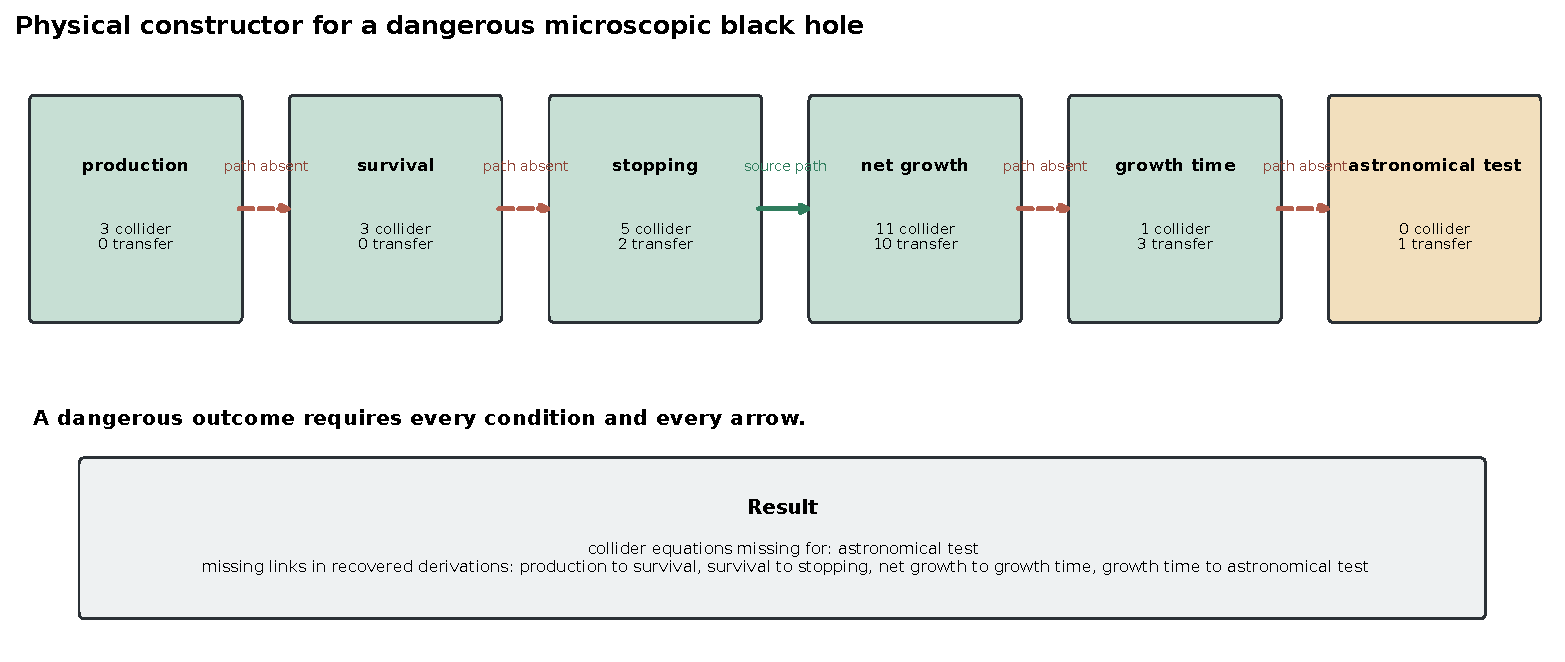
\includegraphics[width=\linewidth]{figures/lhc_physical_constructor.pdf}
\caption{The six gates between a proton collision and a dangerous macroscopic outcome. The ordinary semiclassical branch ends at Gate 2 through Hawking evaporation. The deliberately conservative stable branch continues through stopping and growth calculations, then meets the compact-star observation at Gate 6.}
\label{fig:constructor}
\end{figure}

\section{A catastrophe requires a complete chain}

The feared outcome can be written as a chain in which every condition must be true:
\begin{equation}
\mathcal{D}=P\land S\land C\land G\land T\land A,
\label{eq:danger-chain}
\end{equation}
where $P$ denotes production, $S$ survival, $C$ capture or retention, $G$ positive mass growth, $T$ growth on a relevant timescale, and $A$ compatibility with astronomical observations. The symbol $\land$ means ``and'': if one term fails, the dangerous outcome $\mathcal{D}$ fails. Equation~\eqref{eq:danger-chain} is a logical map rather than a new law of physics. It prevents one dramatic statement, such as ``a black hole might form'', from being mistaken for the complete hazard.

The six terms are coupled. A production model fixes the initial mass and momentum. Those values enter the evaporation and stopping calculations. Stopping determines the material environment in which accretion is evaluated. The mass-growth law must then be integrated over time. Finally, the same production, capture and growth laws must be applied to cosmic-ray collisions with dense astronomical bodies. The conclusion follows from the whole path.

\section{Following the equations}

\subsection{Gate 1: can the collision make a microscopic black hole?}

A proton is composed of quarks and gluons, collectively called partons. Only a fraction of the beam energy enters any one parton-parton collision. The production calculation therefore adds the contributions from every possible pair of partons whose collision energy exceeds the assumed black-hole threshold \cite{GiddingsMangano2008}:
\begin{equation}
\sigma_{\rm BH}(M>M_{\min})=
\sum_{ij}\int_{\tau_{\min}}^1 \ud\tau
\int_\tau^1\frac{\ud x}{x}\,f_i(x)f_j(\tau/x)\,
\hat\sigma(\sqrt{\hat s}).
\label{eq:production}
\end{equation}
Here $\sigma_{\rm BH}$ is the total formation cross-section, which measures production probability. $M$ is black-hole mass, $M_{\min}$ is the minimum mass accepted by the model, $f_i$ and $f_j$ describe the momentum carried by partons of types $i$ and $j$, $x$ is a parton momentum fraction, and $\hat\sigma$ is the formation cross-section for one parton collision. The parton-level energy is $\hat s=x_1x_2s$, where $s$ is the squared proton-proton collision energy. The lower integration limit is
\begin{equation}
\tau=x_1x_2>\tau_{\min}=\frac{M_{\min}^2}{y^2s},
\label{eq:threshold}
\end{equation}
where $y$ is the fraction of collision energy trapped behind the proposed horizon.

\plainmeaning{Equations~\eqref{eq:production} and \eqref{eq:threshold} count quark and gluon collisions energetic enough to cross a hypothetical gravity threshold. They predict production only after a low gravity scale, a minimum mass and a horizon-formation rule have been supplied.}

With the conventional Planck scale, the threshold lies vastly beyond the LHC. Microscopic production at LHC energies belongs to speculative low-scale-gravity models. The remaining five gates test what those models imply if production is granted.

\subsection{Gate 2: does the object survive?}

Hawking radiation makes a small semiclassical black hole lose mass. A retained calculation writes the canonical decay rate as \cite{Koch2008}
\begin{equation}
\frac{\ud M}{\ud t}\approx-c\,\frac{d+1}{4R_{\rm H}^{2}}<0,
\label{eq:evaporation}
\end{equation}
where $M$ is mass, $t$ is time, $c$ is the speed of light, $d$ is the number of extra spatial dimensions in the model, and $R_{\rm H}$ is the horizon radius. The negative sign is the essential result: the black hole shrinks. For a representative mass of ten times the model's fundamental gravity scale, the cited calculation estimates a decay rate at least thirty orders of magnitude larger than the early accretion rate \cite{Koch2008}. CERN summarizes the expected lifetime as about $10^{-27}$~s \cite{CERNExtraDimensions}.

\plainmeaning{The ordinary branch disappears before it can cross a detector, stop in the Earth or begin sustained accretion.}

Safety analyses also examine a stronger hypothetical case in which Hawking evaporation is suppressed or the remnant is stable \cite{GiddingsMangano2008,Plaga2008,Casadio2009}. This assumption keeps the branch alive long enough to test Gates 3 through 6.

\subsection{Gate 3: can matter stop it?}

A stable microscopic black hole produced in a collider would initially move rapidly. It can threaten its surroundings only after interactions remove enough momentum to keep it inside matter. Giddings and Mangano calculate an accretion contribution to the momentum loss per unit path length \cite{GiddingsMangano2008}:
\begin{equation}
\left(\frac{\ud p}{\ud\ell}\right)_{\rm ac}
=-(c_{\rm ac}-c_{\rm ac,M})\,b_{\min}^{2}\pi\rho
\frac{E^{2}}{M^{2}}R^{2}(\sqrt{s_{\rm int}}).
\label{eq:stopping}
\end{equation}
Here $p$, $E$ and $M$ are the black hole's momentum, energy and mass; $\ell$ is distance travelled; $\rho$ is the energy density of the material; $R$ is the gravitational capture radius; $s_{\rm int}$ is the squared centre-of-mass energy for the black-hole/constituent encounter; $b_{\min}R$ is the limiting impact parameter for capture; and $c_{\rm ac}$ and $c_{\rm ac,M}$ describe the fractions of momentum and energy transferred in an encounter.

\plainmeaning{The equation accumulates many tiny interactions along a path. If the integrated momentum loss is smaller than the momentum needed to escape, the object leaves the Earth. If it is retained, its final speed and location set the initial conditions for accretion.}

This gate is especially important for the astronomical comparison. Black holes hypothetically produced by cosmic rays can be much more strongly boosted than products at a symmetric collider. A useful natural test therefore requires an object dense enough to stop some of them. White dwarfs and neutron stars provide that test.

\subsection{Gate 4: does it gain mass faster than it loses mass?}

For motion through matter, a primary source gives the capture law \cite{GiddingsMangano2008}
\begin{equation}
\left.\frac{\ud M}{\ud t}\right|_{\rm acc}=\pi\rho v r_c^2(M),
\label{eq:accretion}
\end{equation}
where $v$ is speed through the material and $r_c(M)$ is the mass-dependent capture radius. A second source makes the competition explicit \cite{Casadio2009}:
\begin{equation}
\frac{\ud M}{\ud t}=
\left.\frac{\ud M}{\ud t}\right|_{\rm evap}+
\left.\frac{\ud M}{\ud t}\right|_{\rm acc}.
\label{eq:balance}
\end{equation}

\plainmeaning{The area $\pi r_c^2$ sets how much material is intercepted. Multiplying it by density $\rho$ and speed $v$ gives the incoming mass rate. Growth begins only when this gain remains larger than evaporation and other losses.}

A positive value at one instant does not establish catastrophe. The density, velocity and capture radius change as the object slows and grows. The full trajectory leads to Gate 5.

\subsection{Gate 5: can growth finish within the available time?}

The time needed to grow from an initial mass $M_0$ to a larger mass $M_*$ follows from the net mass rate:
\begin{equation}
t_{\rm grow}(M_0\!\rightarrow\!M_*)=
\int_{M_0}^{M_*}\frac{\ud M}{\dot M_{\rm net}(M)}.
\label{eq:growth-time}
\end{equation}
Here $\dot M_{\rm net}$ is the right-hand side of Eq.~\eqref{eq:balance}. The source calculations split the integral into regimes because the relevant capture radius changes with mass. For a six-dimensional white-dwarf model, one recovered system is \cite{GiddingsMangano2008}
\begin{align}
t(R_B<R_D)&=\frac{8}{\lambda_6}\left(\frac{M_D}{M_0}\right)^2\yr,\nonumber\\
t(R_D<R_B<R_C)&=\frac{4\times10^2}{\lambda_4}\left(\frac{M_D}{M_0}\right)^2\yr,\nonumber\\
t(R_B>R_C)&=\frac{15}{\lambda_4}\left(\frac{M_D}{M_0}\right)^2\yr.
\label{eq:white-dwarf-times}
\end{align}
$R_B$ is the Bondi radius at which gravity organizes the surrounding flow, $R_D$ marks the end of the higher-dimensional regime, $R_C$ marks the transition to four-dimensional gravity, $M_D$ is the fundamental gravity scale, and $\lambda_4$ and $\lambda_6$ are dimension-dependent accretion coefficients. In the seven-dimensional cases considered in the same paper, the longest relevant white-dwarf stage remains below about 80 million years, while known white dwarfs live for more than a billion years \cite{GiddingsMangano2008}.

\plainmeaning{A local tendency to grow is converted into a clock. Any model that predicts rapid terrestrial growth also predicts an observable compact-star consequence on a much shorter timescale than the star's age.}

\subsection{Gate 6: what do compact stars tell us?}

Cosmic rays reach laboratory energies far above the LHC beam energy and have struck planets and stars for billions of years \cite{CERNCosmicRays,Ellis2008}. A cosmic ray hits a nearly stationary target, so only part of its laboratory energy enters the centre-of-mass collision; the highest-energy events still cover and exceed the LHC-relevant range. Under a stable-black-hole hypothesis, some collisions should therefore produce the same species considered at the LHC. Dense compact stars are effective detectors because they provide enormous column density and long exposure. One recovered warped-model calculation gives
\begin{equation}
t_{\rm NS,w}\sim20\,\yr,
\label{eq:neutron-star}
\end{equation}
where $t_{\rm NS,w}$ is the predicted neutron-star growth time in that model \cite{GiddingsMangano2008}. Neutron stars survive far longer than twenty years. White-dwarf calculations provide the same form of test over longer, model-dependent intervals.

The observation is stronger than a verbal analogy. Production, momentum loss, capture radius, density and growth time are recalculated for the star. A model that predicts production, capture and destructive growth must reproduce the continued existence of the objects that have already hosted the natural collisions.

\section{What two maps of the literature reveal}

Scientific papers carry two different kinds of structure. Citations, authors and stated conclusions show how an argument travelled. Equations show how one physical quantity is converted into another. We built both maps from the same sources.

The Hyperion operational archive contains 2.5 million arXiv papers. The fixed public LHC experiment scanned @@SCANNED_COUNT@@ source documents and selected @@SELECTED_COUNT@@ records using terms connected to colliders, black holes, cosmic rays, compact stars, evaporation and accretion. Six complete primary safety papers were then added, producing @@SOURCE_COUNT@@ unique paper nodes. The broad set intentionally includes neighboring astrophysics because the stopping and growth laws are developed there. The six primary papers carry the quantitative LHC safety argument.

The provenance graph contains @@CLAIM_COUNT@@ extracted claim nodes, @@REFERENCE_COUNT@@ cited-paper nodes, @@CITATION_LINKS@@ citation links and @@CLAIM_LINKS@@ paper-to-claim links. Figure~\ref{fig:provenance-summary} reduces it to its main families. Risk claims, safety claims and astronomical statements all occur. Their counts describe the discussion; the equations decide whether the feared chain is physically closed.

\begin{figure}[H]
\centering
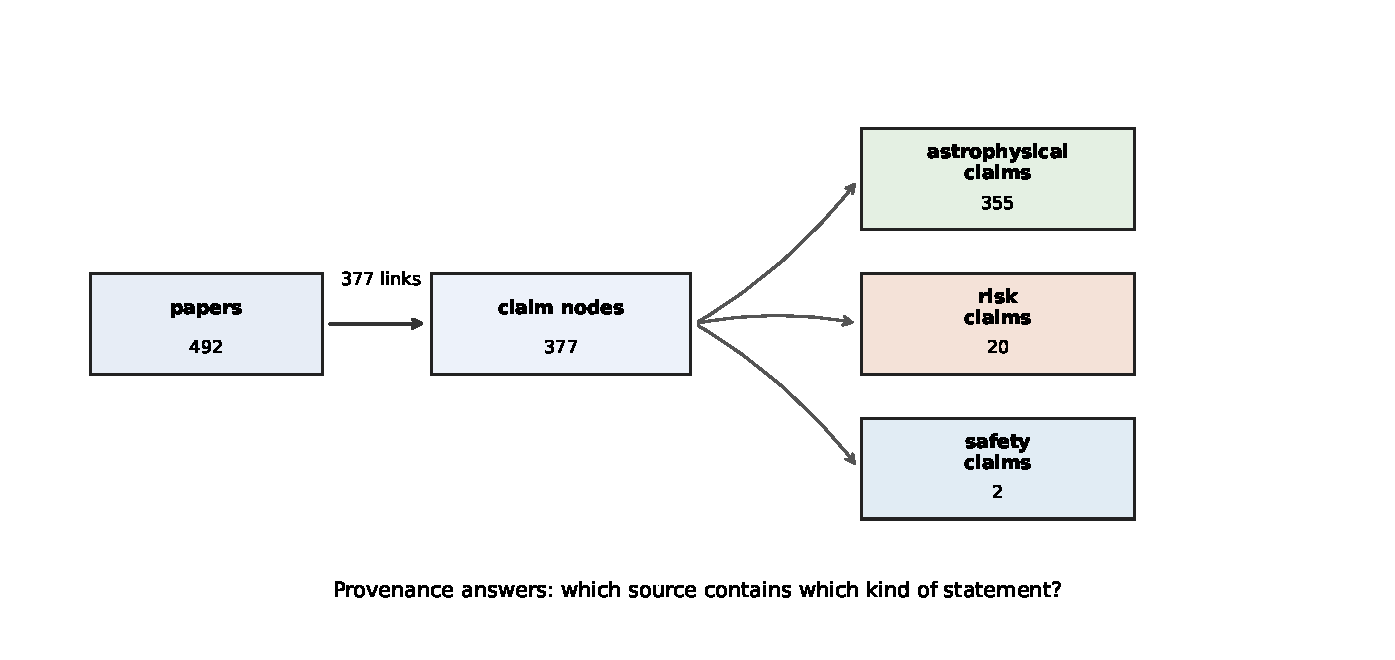
\includegraphics[width=0.96\linewidth]{figures/lhc_provenance_summary.pdf}
\caption{The provenance map records where claims came from and how papers cite one another. The three claim families coexist in the search set. Their presence identifies the dispute; it does not combine their physical assumptions.}
\label{fig:provenance-summary}
\end{figure}

\begin{figure}[H]
\centering
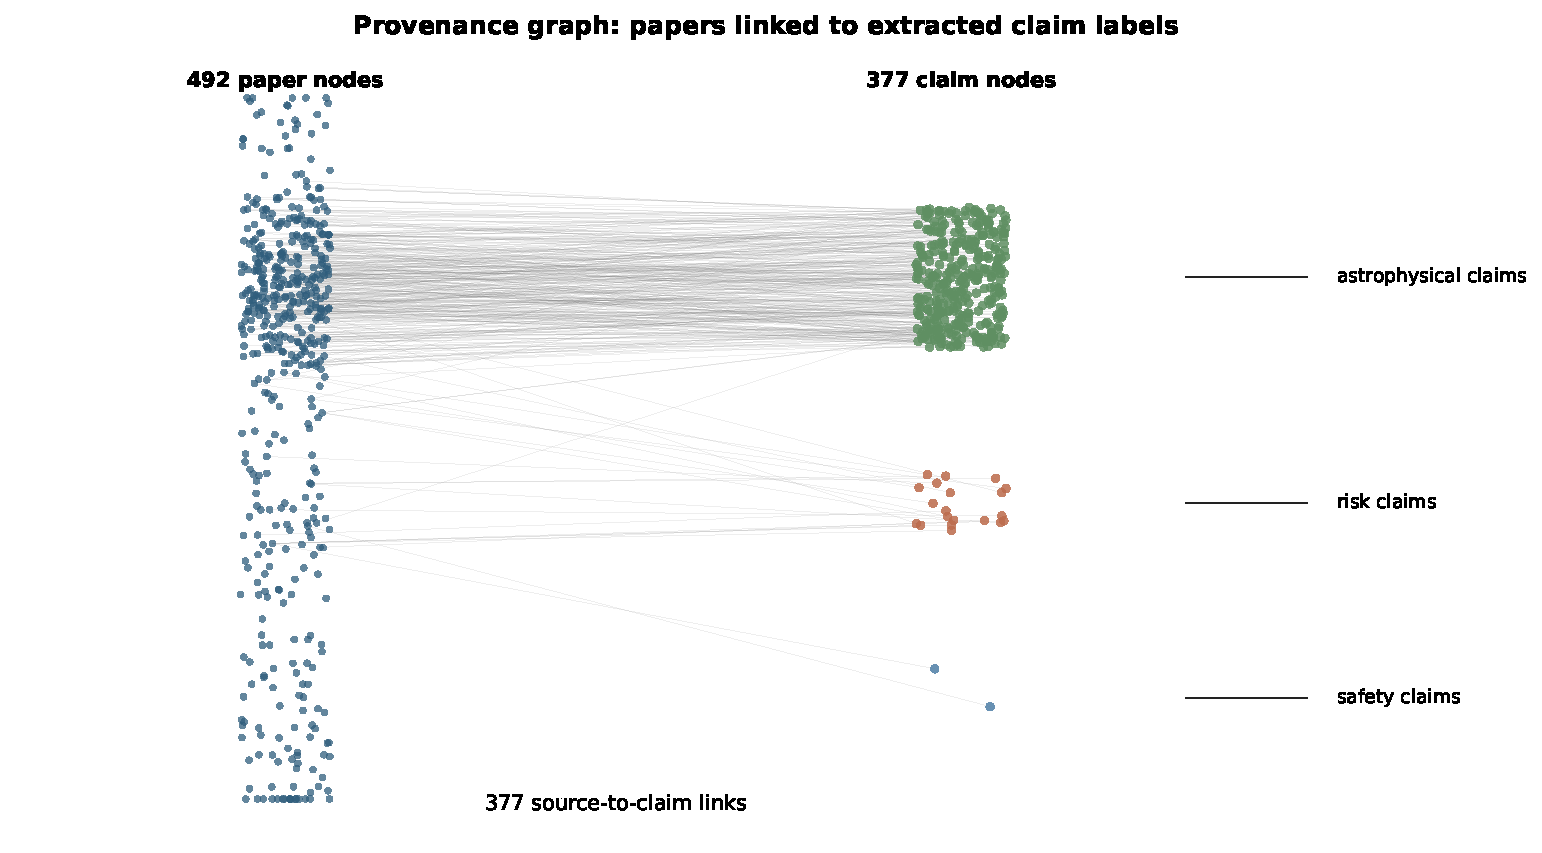
\includegraphics[width=\linewidth]{figures/lhc_provenance_full.pdf}
\caption{The complete provenance graph used in this reconstruction. Each point is a named author, selected paper, cited paper or extracted claim. Outlined points identify the six complete primary papers used for the equation benchmark.}
\label{fig:provenance}
\end{figure}

The equation graph starts from @@EQUATION_WINDOW_COUNT@@ equations together with their positions and nearby text. The software converted @@GRAPH_NODE_COUNT@@ into numerical descriptions of the operation being performed; @@USABLE_NODE_COUNT@@ contained enough information to identify a physical role. It then found @@GRAPH_EDGE_COUNT@@ equation-to-equation steps inside individual papers and @@ANALOG_EDGE_COUNT@@ candidate matches between different papers. Each retained node records the source equation, the quantities it consumes and produces, its physical setting and its position in the paper.

Figure~\ref{fig:equation-graph} organizes the @@STRICT_RECEIPT_COUNT@@ distinct equations that satisfy at least one of the six physical conditions. Circles mark equations written in collider or LHC-safety contexts. Diamonds mark equations from material or astrophysical settings that calculate the same physical quantity and therefore supply a transfer test.

\begin{figure}[H]
\centering
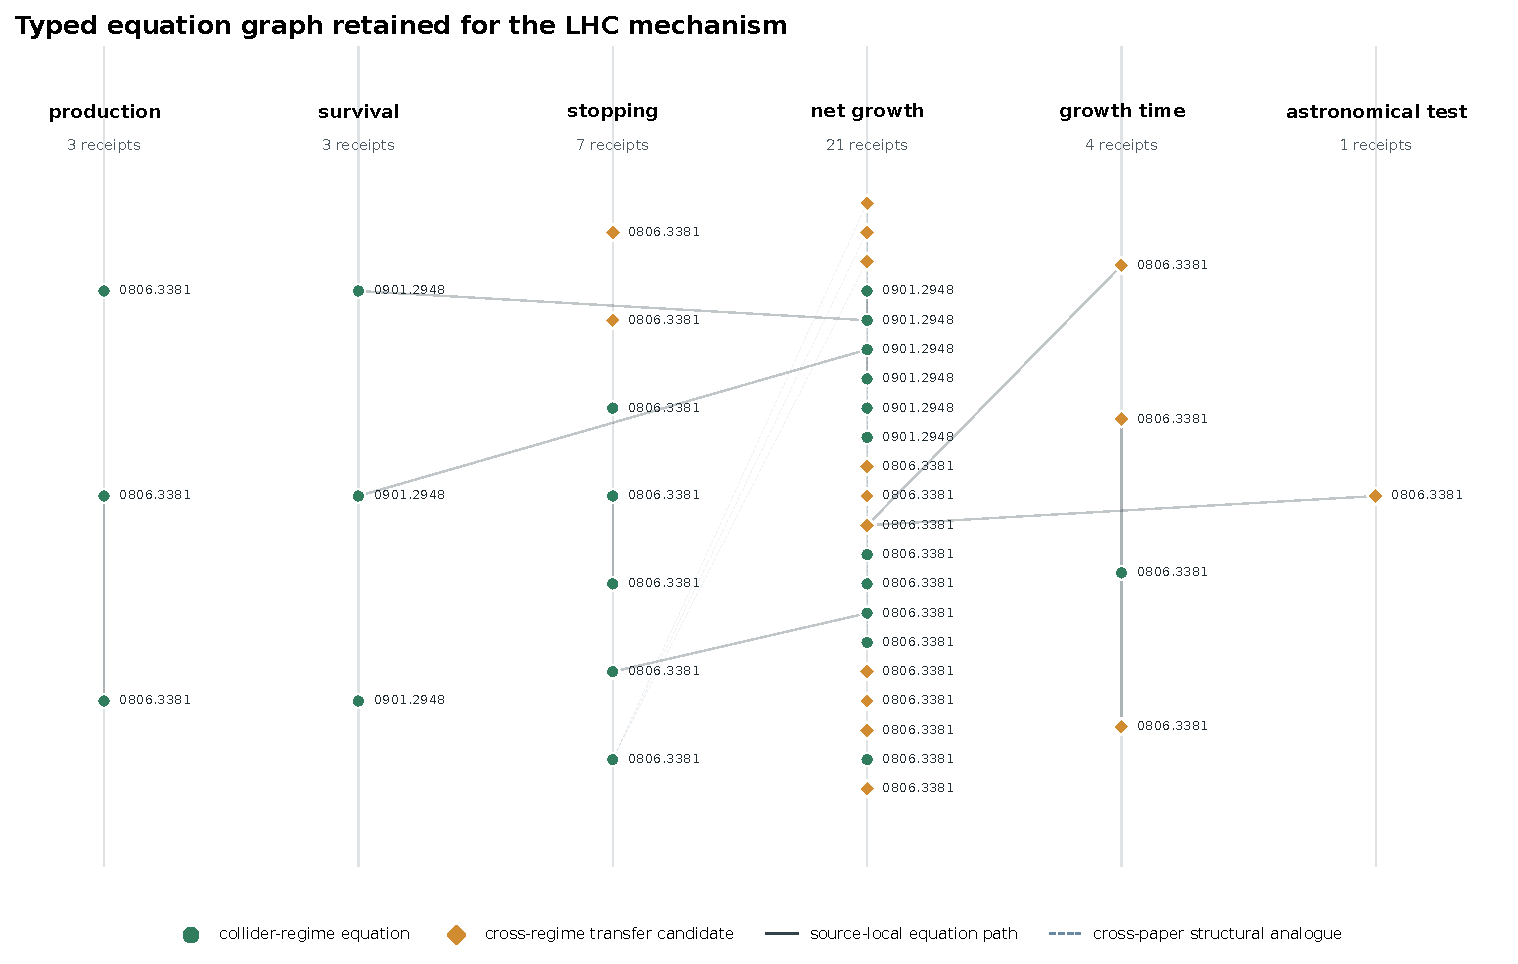
\includegraphics[width=\linewidth]{figures/lhc_equation_graph.pdf}
\caption{The equation-level mechanism graph. Columns are the six necessary physical conditions. Solid lines preserve source order inside a paper; dashed lines join equations that perform the same mathematical operation in different papers. The graph exposes where the literature provides a derivation and where separate model assumptions must be combined.}
\label{fig:equation-graph}
\end{figure}

\begin{table}[H]
\centering
\caption{Equations assigned to each necessary condition. A single equation can contribute to more than one condition, so column totals are assignments rather than unique papers.}
\label{tab:constructor}
\begin{tabularx}{\linewidth}{YrrY}
\toprule
Condition & Direct equations & Transfer equations & Quantity calculated \\
\midrule
@@SLOT_TABLE@@
\bottomrule
\end{tabularx}
\end{table}

The graph makes the result precise. Equations cover every local process, and @@DIRECT_ASSIGNMENTS@@ direct assignments connect primary-source equations to collider conditions. @@CANDIDATE_ASSIGNMENTS@@ assignments carry stopping, growth or astronomical calculations across physical settings. Within the papers, the equations directly connect stopping to mass growth. No single derivation carries one consistent parameter set through production, survival, stopping, growth time and the compact-star test. The literature is modular: one paper grants stability to study its consequences, another evaluates Hawking loss, and another computes capture under a particular dimensional model.

Two positive results recovered from the equations determine the physical conclusion. The standard semiclassical branch has a large negative mass rate. The stable branch predicts compact-star effects when growth is fast enough to matter on Earth. These results close the dangerous route from opposite sides.

\begin{figure}[H]
\centering
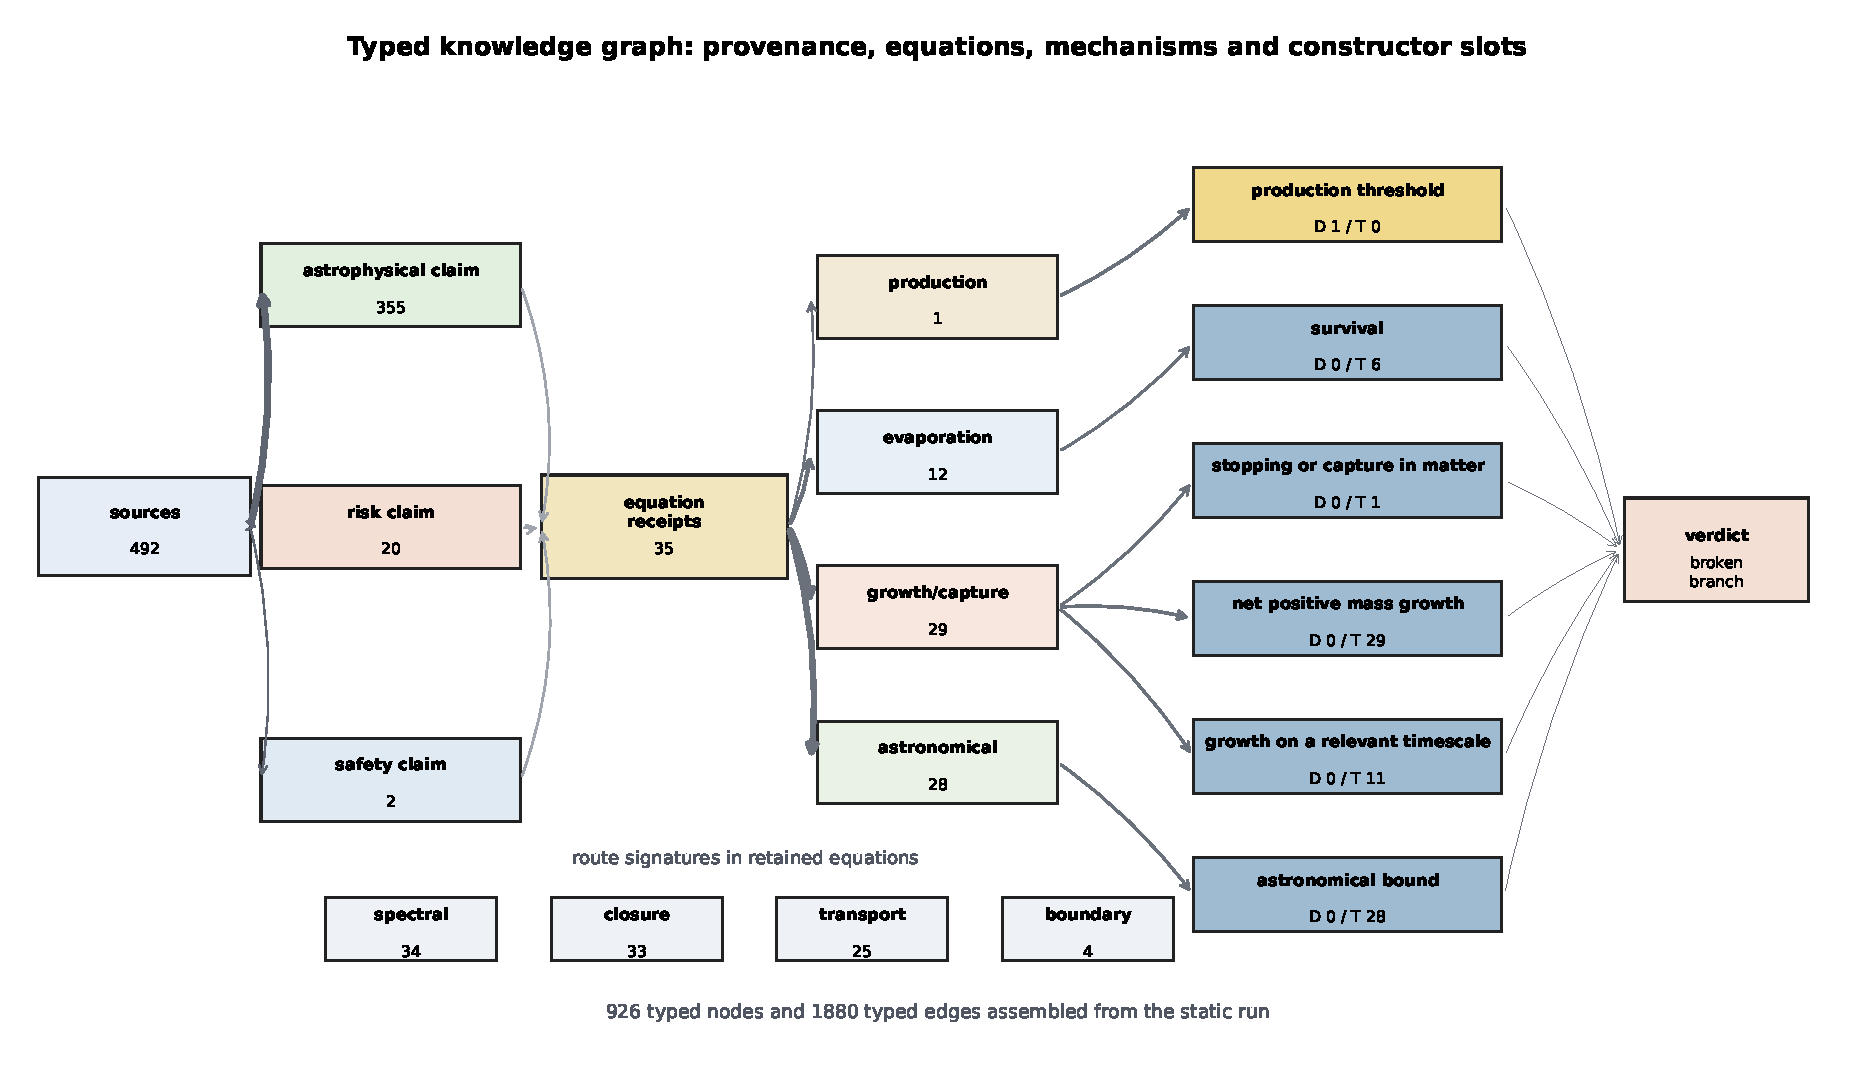
\includegraphics[width=\linewidth]{figures/lhc_public_knowledge_graph.pdf}
\caption{The joined graph connects source history to physical calculation. Brown links carry authorship, citation and claims. Green links run from papers through equations and calculation types to the six conditions and the final answer.}
\label{fig:joined}
\end{figure}

\section{How an equation from a star becomes evidence about a collider}

The transfer from astrophysics to collider safety preserves a physical question while changing the environment. Consider Eq.~\eqref{eq:accretion}. The mass rate always depends on density $\rho$, speed $v$ and capture radius $r_c$. A white dwarf and the Earth have different values of all three. The equation remains the same; its parameters are recomputed.

Figure~\ref{fig:transfer} shows four transfers recovered in the case graph. The middle column states the quantity that must be preserved: momentum loss, net mass rate, integrated growth time or an astronomical survival bound. The right column states the collider-specific test. This step blocks a common error in qualitative arguments, where a formula is moved between environments without changing its boundary conditions or parameter ranges.

\begin{figure}[H]
\centering
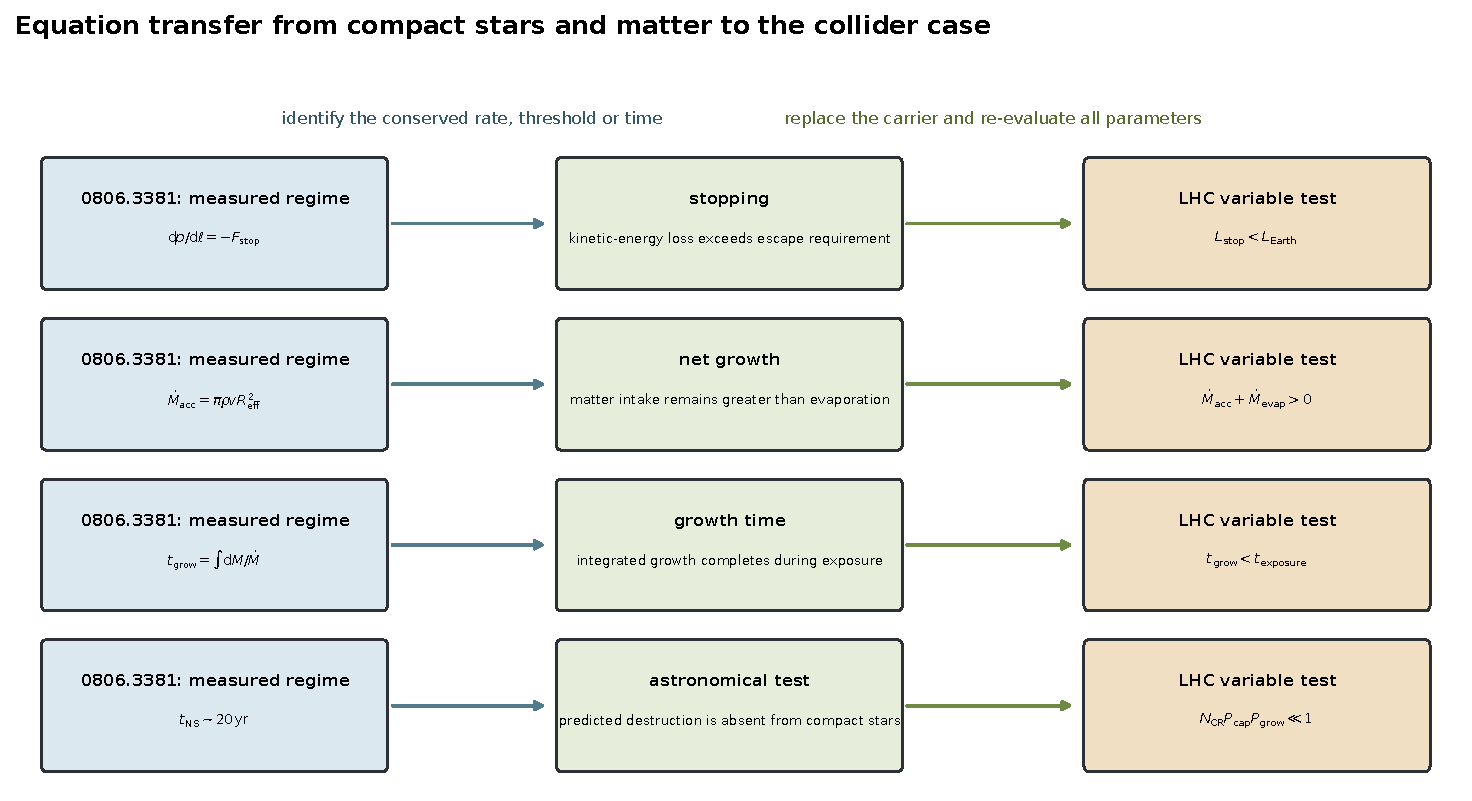
\includegraphics[width=\linewidth]{figures/lhc_transfer_map.pdf}
\caption{Equation transfer between physical environments. The mathematical role is held fixed while density, velocity, size, exposure and initial conditions are replaced. The transferred relation becomes evidence after dimensions, parameter ranges and boundary conditions agree.}
\label{fig:transfer}
\end{figure}

\section{How the reconstruction was made}

The procedure has five steps. First, displayed equations and their nearby sentences are extracted from each LaTeX source. Second, every equation receives a numerical description, called a fingerprint, of its mathematical operation and physical quantities: threshold, rate, transport, constraint, boundary condition or ordered step. Third, equations are linked in their order of appearance inside each source. Equations that perform the same mathematical operation in different papers form candidate transfer links. Fourth, six explicit equation tests are applied. A stopping equation must contain a momentum or energy loss over distance; a growth equation must contain a mass rate; a timescale equation must integrate or evaluate that rate. Fifth, the resulting graph is searched for paths that pass the six gates while preserving compatible quantities and physical settings.

This is how the method separates a repeated phrase from a physical dependency. The phrase ``stable microscopic black hole'' can appear in many claims. It contributes to the mechanism only when a source supplies a lifetime assumption and then carries the resulting mass and momentum into stopping or growth equations.

\begin{figure}[H]
\centering
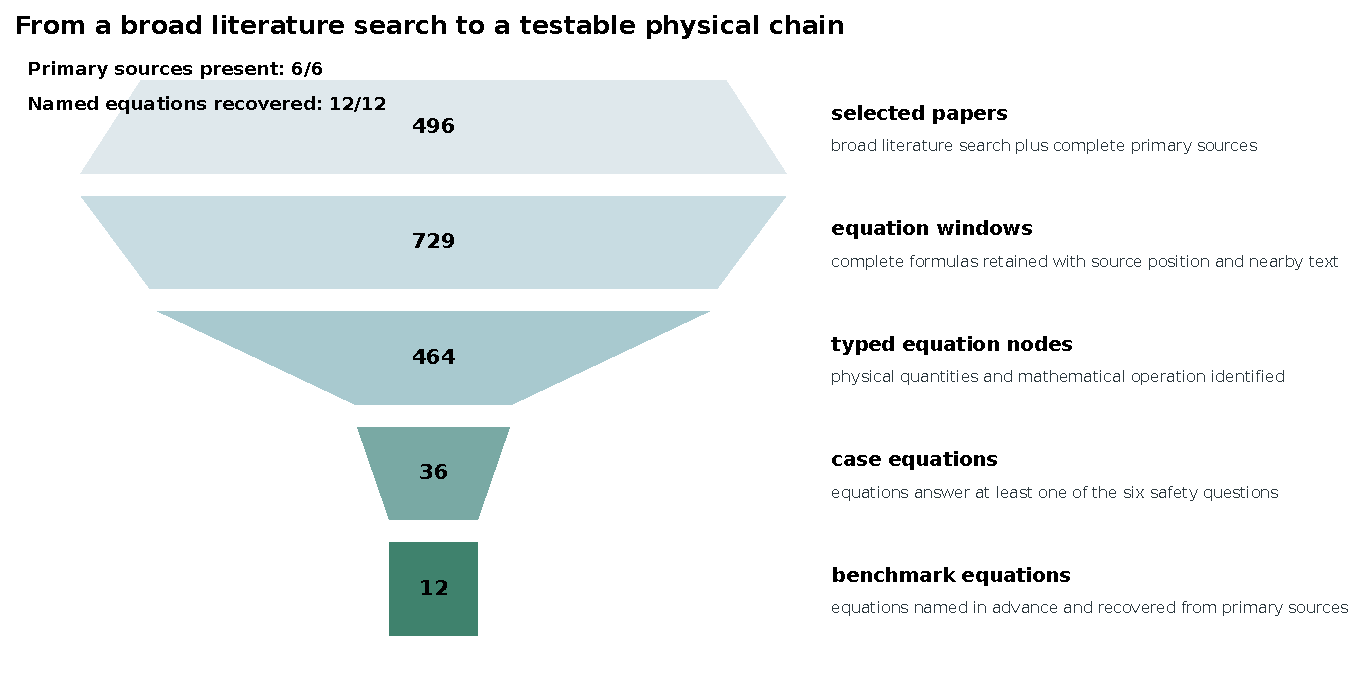
\includegraphics[width=0.94\linewidth]{figures/lhc_evidence_funnel.pdf}
\caption{From broad literature to equations used in the physical chain. The last stage is a benchmark of named equations selected before the final mechanism graph was assembled.}
\label{fig:funnel}
\end{figure}

\subsection{A direct check against the primary sources}

Twelve equations were named in advance across the six primary papers. They cover production, the parton threshold, Hawking loss, stopping, accretion, competing mass rates, growth stages and compact-star bounds. The extraction recovered @@RECOVERED_RECEIPTS@@ of @@TOTAL_RECEIPTS@@ and each passed its prespecified equation test.

\begin{table}[H]
\centering
\caption{Primary-source equation recovery. Review and response papers contain fewer calculation equations; the main calculation papers supply the named tests.}
\label{tab:gold}
\begin{tabular}{lrr}
\toprule
arXiv source & Extracted equations & Named equations recovered \\
\midrule
@@SOURCE_TABLE@@
\bottomrule
\end{tabular}
\end{table}

\subsection{Which transitions carry the argument?}

The graph ranking gives greater weight to an uncommon, informative equation-to-equation step than to a connection repeated throughout the corpus. Its strongest individual step is @@TOP_TRANSITION@@. Across the high-ranking links, three operations dominate in ordinary physical terms: an equation defines an allowed range, another propagates mass or momentum, and a constraint tests the result. This is the mathematical skeleton of the safety argument. Repetition of a conclusion does not raise this score.

\begin{figure}[H]
\centering
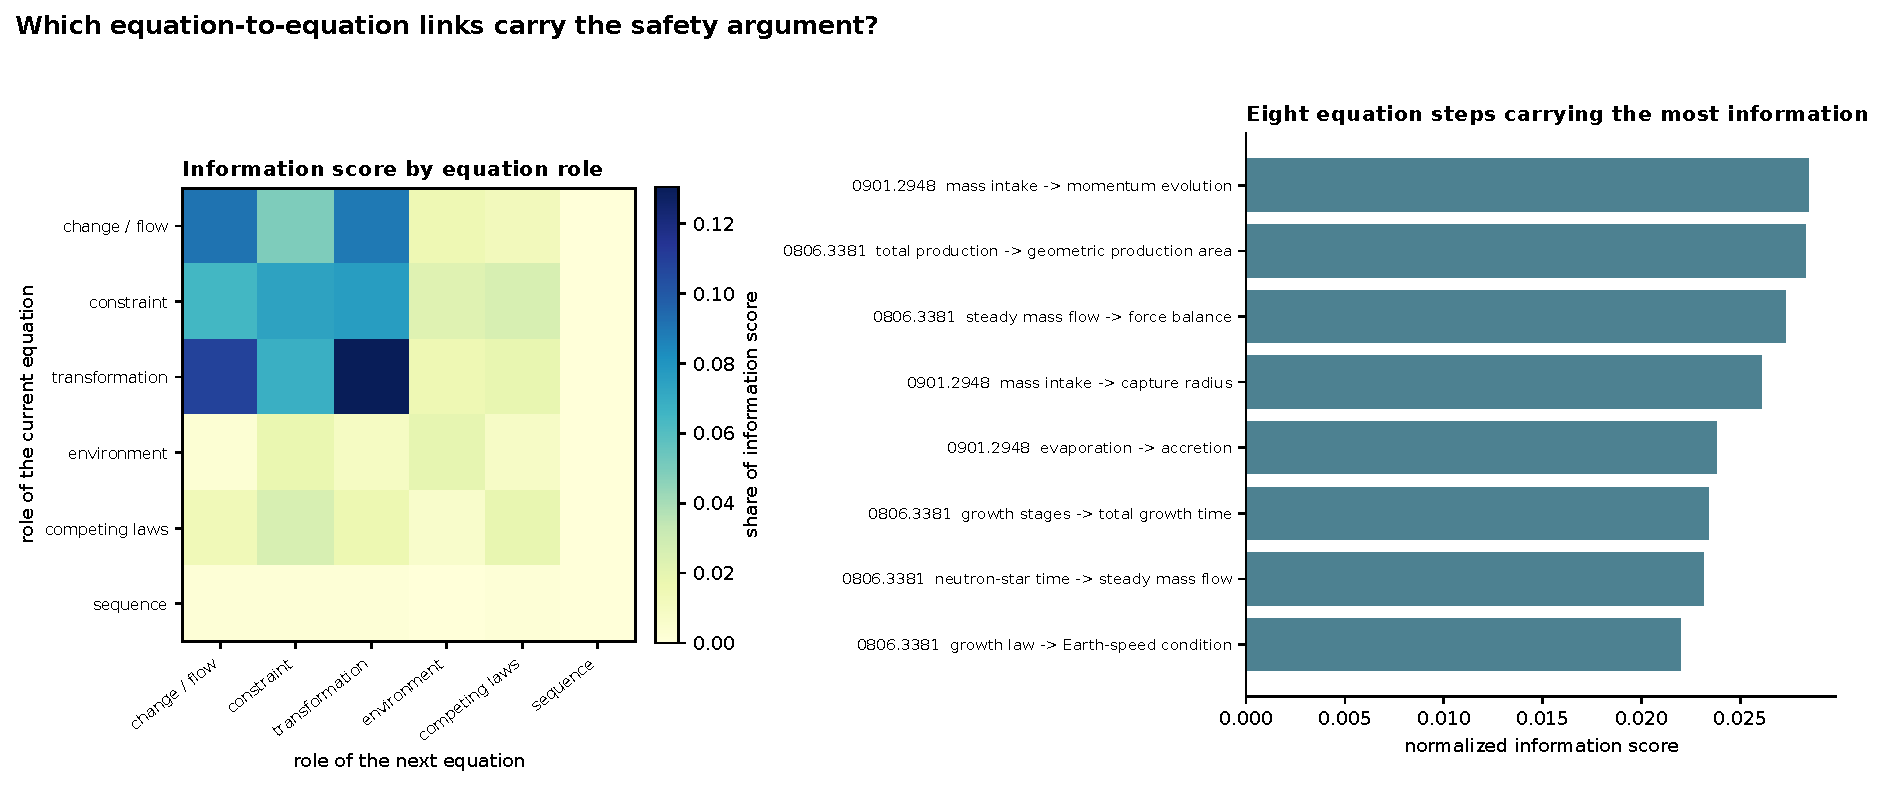
\includegraphics[width=0.96\linewidth]{figures/lhc_sparse_attention.pdf}
\caption{Information carried by equation-to-equation transitions. The matrix groups transitions by mathematical role; the bars show the individual source transitions that contribute most strongly. High rank identifies a useful dependency, rather than a popular claim.}
\label{fig:sparse}
\end{figure}
\FloatBarrier

\section{Independent comparison with the CERN safety report}

CERN-2003-001 was written by the LHC Safety Study Group before operation of the collider \cite{CERN2003}. It was excluded from the arXiv equation corpus and from the twelve-equation benchmark. The report therefore provides an independent human reconstruction.

The agreement is specific. Both analyses begin by making microscopic production conditional on speculative low-scale gravity. Both separate the rapidly evaporating branch from a stable hypothetical branch. Both carry the stable branch through stopping and accretion. Both use cosmic-ray exposure and the survival of astronomical bodies as the final test. The later peer-reviewed LHC safety review follows the same structure \cite{Ellis2008}.

\begin{table}[H]
\centering
\caption{Independent comparison of the automatically reconstructed chain with CERN-2003-001.}
\begin{tabularx}{\linewidth}{Y Y Y}
\toprule
Physical question & Automated reconstruction & CERN safety report \\
\midrule
Can microscopic production occur? & Conditional on a low gravity scale and threshold & Treated as a speculative model branch \\
What happens to the ordinary branch? & Hawking mass loss ends the branch & Rapid decay ends the branch \\
How is a stable branch tested? & Momentum loss, capture and accretion & Stopping and accretion calculations \\
What supplies the long-exposure test? & Cosmic rays, white dwarfs and neutron stars & Natural cosmic-ray collisions and surviving bodies \\
Case conclusion & No closed dangerous mechanism & No conceivable threat \\
\bottomrule
\end{tabularx}
\end{table}

The independent match covers the order of the argument, the decisive physical quantities and the final result. It also identifies what the automated graph adds: every step can be traced to a source equation, its variables and the regime in which it was derived.

\section{Conclusion}

The LHC black-hole question has a clear physical answer. Conventional gravity does not place microscopic black-hole production within LHC reach. Low-scale-gravity models can make production calculable, but their ordinary black holes evaporate almost immediately. Granting stability moves the burden to stopping, net mass growth and growth time. Models that make this branch fast enough to threaten the Earth also predict observable consequences in compact stars exposed to LHC-relevant natural collisions over vastly longer times. Those stars survive.

The broad literature contains risk statements, safety statements and many neighboring astrophysical calculations. Their physical content becomes clear when equations are assembled in causal order. Production is an entrance condition, evaporation is an early exit, stopping supplies initial conditions for accretion, integration turns a rate into a timescale, and compact stars test the completed stable branch. No equation-supported path in the processed literature reaches a dangerous macroscopic outcome.

The same representation can be updated locally. A new evaporation law would alter Gate 2. A new capture calculation would alter Gate 3. A newly observed compact-star population would strengthen or narrow Gate 6. The answer remains attached to the physical quantities that determine it.

\begin{thebibliography}{12}
\bibitem{CERNFAQ} CERN, ``The Large Hadron Collider: frequently asked questions,'' \url{https://home.cern/resources/faqs/large-hadron-collider-dangerous}.
\bibitem{CERNExtraDimensions} CERN, ``Extra dimensions, gravitons, and tiny black holes,'' \url{https://home.cern/science/physics/extra-dimensions-gravitons-and-tiny-black-holes/}.
\bibitem{CERNCosmicRays} CERN, ``Cosmic rays: particles from outer space,'' \url{https://home.cern/science/physics/cosmic-rays-particles-outer-space/}.
\bibitem{CERN2003} J.-P. Blaizot et al., ``Study of potentially dangerous events during heavy-ion collisions at the LHC: Report of the LHC Safety Study Group,'' CERN-2003-001 (2003), \url{https://cds.cern.ch/record/613175/files/CERN-2003-001.pdf}.
\bibitem{ADD1998} N. Arkani-Hamed, S. Dimopoulos and G. Dvali, ``The hierarchy problem and new dimensions at a millimeter,'' Phys. Lett. B 429, 263--272 (1998), \url{https://arxiv.org/abs/hep-ph/9803315}.
\bibitem{GiddingsThomas2002} S. B. Giddings and S. Thomas, ``High energy colliders as black hole factories: the end of short distance physics,'' Phys. Rev. D 65, 056010 (2002), \url{https://arxiv.org/abs/hep-ph/0106219}.
\bibitem{DimopoulosLandsberg2001} S. Dimopoulos and G. Landsberg, ``Black holes at the Large Hadron Collider,'' Phys. Rev. Lett. 87, 161602 (2001), \url{https://arxiv.org/abs/hep-ph/0106295}.
\bibitem{GiddingsMangano2008} S. B. Giddings and M. L. Mangano, ``Astrophysical implications of hypothetical stable TeV-scale black holes,'' Phys. Rev. D 78, 035009 (2008), \url{https://arxiv.org/abs/0806.3381}.
\bibitem{Ellis2008} J. Ellis et al., ``Review of the Safety of LHC Collisions,'' J. Phys. G 35, 115004 (2008), \url{https://arxiv.org/abs/0806.3414}.
\bibitem{Koch2008} B. Koch, M. Bleicher and H. Stoecker, ``Exclusion of black hole disaster scenarios at the LHC,'' Phys. Lett. B 672, 71--76 (2009), \url{https://arxiv.org/abs/0807.3349}.
\bibitem{Plaga2008} R. Plaga, ``On the potential catastrophic risk from metastable quantum-black holes produced at particle colliders,'' \url{https://arxiv.org/abs/0808.1415}.
\bibitem{Casadio2009} R. Casadio, S. Fabi and B. Harms, ``Possibility of catastrophic black hole growth in the warped brane-world scenario at the LHC,'' \url{https://arxiv.org/abs/0901.2948}.
\end{thebibliography}

\end{document}
